% !Mode:: "TeX:ACP:Hard"
\documentclass[14pt,hyperref={CJKbookmarks=true}]{beamer}

%\usepackage[space,noindent]{ctex}
\usepackage{mathrsfs}
\usepackage{amsfonts,amssymb}
\usepackage{amsmath}
\usepackage{graphicx}
\usepackage{subcaption}
\usepackage{lmodern}
\usepackage[labelformat=empty,font=scriptsize,skip=0pt,justification=centering,singlelinecheck=false]{caption}
\usepackage{bibentry}
\usepackage{csquotes}
\usepackage{amsthm}
\usepackage{color}
\theoremstyle{plain}
\usepackage{booktabs}
\newtheorem{thm}{Theorem}[section]
\newtheorem{lem}[thm]{Lemma}
\newtheorem{prop}[thm]{Proposition}
\newtheorem*{cor}{Corollary}

\theoremstyle{definition}
\newtheorem{defn}{Definition}[section]
\newtheorem{conj}{Conjecture}[section]
\newtheorem{exmp}{Example}[section]

\theoremstyle{remark}
\newtheorem*{rem}{Remark}

%\captionsetup{font={scriptsize}}
\captionsetup[figure]{name=Fig., labelsep=space}
%remove the icon
\setbeamertemplate{bibliography item}{}
%remove line breaks
\setbeamertemplate{bibliography entry title}{}
\setbeamertemplate{bibliography entry location}{}
\setbeamertemplate{bibliography entry note}{}
\usetheme{AnnArbor}
%\usetheme{CambridgeUS}
%\usetheme{Berlin}
%\usetheme{Dresden}
%\usecolortheme{beaver}
%\setbeamercolor{itemize item}{fg=black!80!black}
\usefonttheme{serif}     % Font theme: serif
\usepackage{ccfonts}     % Font family: Concrete Math
\usepackage[T1]{fontenc} % Font encoding: T1
\setbeamercolor{normal text}{bg=black!10}
\setbeamerfont{caption}{size=\tiny}
\graphicspath{{./image/}}
\setlength\itemsep{0em}
\begin{document}

%\section{Title}


\title[IACAS]{Filter and its Applications}
%\subtitle[副题简称]{论文副题}
\author{Tian Chen}
\institute[]{Institute of Automation, Chinese Academy of Sciences\\University of Chinese Academy of Sciences}
\date[]{2017.05.25}


\begin{frame}
\titlepage
\end{frame}


%% Outline page
\begin{frame}
\frametitle{Quick Overview}
\small\tableofcontents
\end{frame}


%%%\caption{Classification of System}
\section{Introduction}
\frame{\tableofcontents[currentsection]}

%\begin{block}{R.E.Kalman(1930-2016)}
%%%%%%%%figure of kalman
\begin{frame}
\frametitle{R. E. Kalman}
\small
\begin{figure}
\centering
\begin{minipage}[t]{0.3\textwidth}
\centering
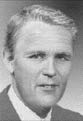
\includegraphics[width=2cm,height=3cm]{kalman0.jpg}
\end{minipage}
\begin{minipage}[t]{0.3\textwidth}
\centering
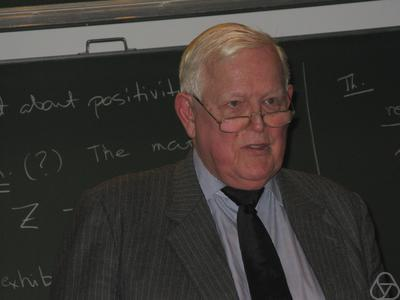
\includegraphics[width=4cm,height=3cm]{kalman.jpg}
\end{minipage}
\caption{\\Born 1930 in Hungry\\
Studied at MIT/Columbia\\
Developed filter in 1960/61}
\label{fig:graph}
\end{figure}
\begin{displayquote}\scriptsize
His passing not only brought about personal loss but also a sad  reminder of the passing of a golden era in systems and control.

\hfill --Yu-Chi Ho
\end{displayquote}

\end{frame}

\begin{frame}
\small \frametitle{Kalman Filter}
\begin{itemize}
\item Kalman filtering has proved useful in navigational and guidance systems, radar tracking, sonar ranging, and satellite orbit determination, to name just a few areas. 
\item Kalman and Bucy's original papers have generated thousands of other papers on aspects and applications of filtering. Their work has also stimulated mathematical research in such areas as numerical methods for linear algebra.
\end{itemize}
\end{frame}


\begin{frame}
\small \frametitle{Particle Filter}
\begin{itemize}
\item {\bf{First attempts-simulations of growing polymers}}
\item[-] Rosenbluth M N, Rosenbluth A W. Monte Carlo Calculation of the Average Extension of Molecular Chains[J]. Journal of Chemical Physics, 1955, 23(2):356-359.
\item {\bf{First application in signal processing-1993}}
\item[-] Gordon N J, Salmond D J, Smith A F M. Novel approach to nonlinear/non-Gaussian Bayesian state estimation[J]. IEE Proceedings F - Radar and Signal Processing, 2002, 140(2):107-113.
\end{itemize}
\end{frame}



\section{Filter}
\frame{\tableofcontents[currentsection]}

\subsection{State Space Model}



\begin{frame}
\frametitle{Linear State Space Model}
\begin{table}
\small
\begin{tabular}{c c c}
\toprule[1pt]
process & Linear Process & Nonliear Process\\
\midrule[0.5pt]
motion model &$\mathbf{A}_{k}\mathbf{x}_{k-1}+\mathbf{B}_{k}\mathbf{u}_{k}+\mathbf{q}_{k}$ & $\mathbf{f}(\mathbf{x}_{k-1},\mathbf{u}_{k},\mathbf{q}_{k})$\\
observation model &  $\mathbf{H}_k\mathbf{x}_k+\mathbf{r}_k$ &  $\mathbf{g}(\mathbf{x}_k,\mathbf{r}_k)$ \\
Estimation & kalman Filter& EKF, Particle Filter\\
\bottomrule[1pt]
\end{tabular}
\end{table}
\begin{figure}
\centering
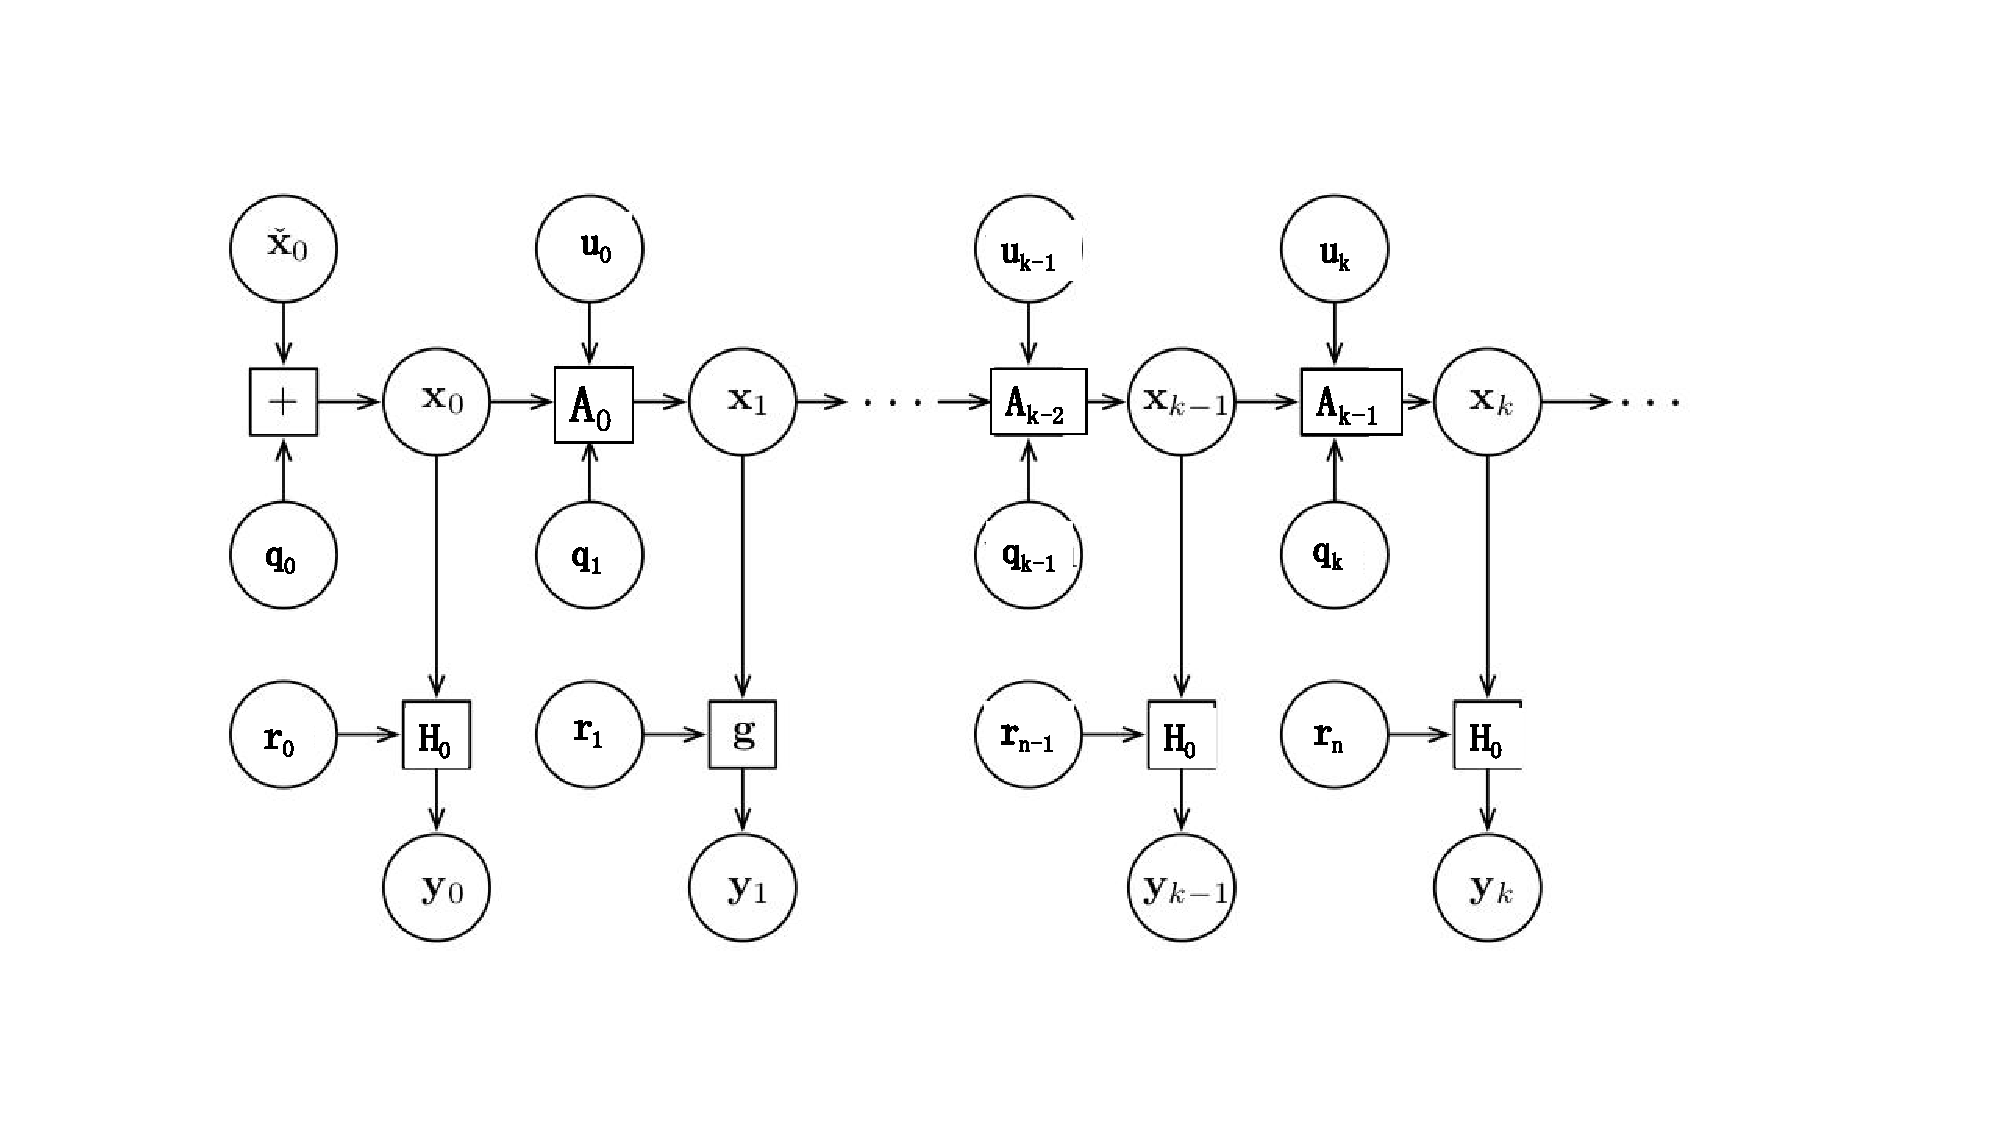
\includegraphics[width=0.45\linewidth]{state1.pdf}
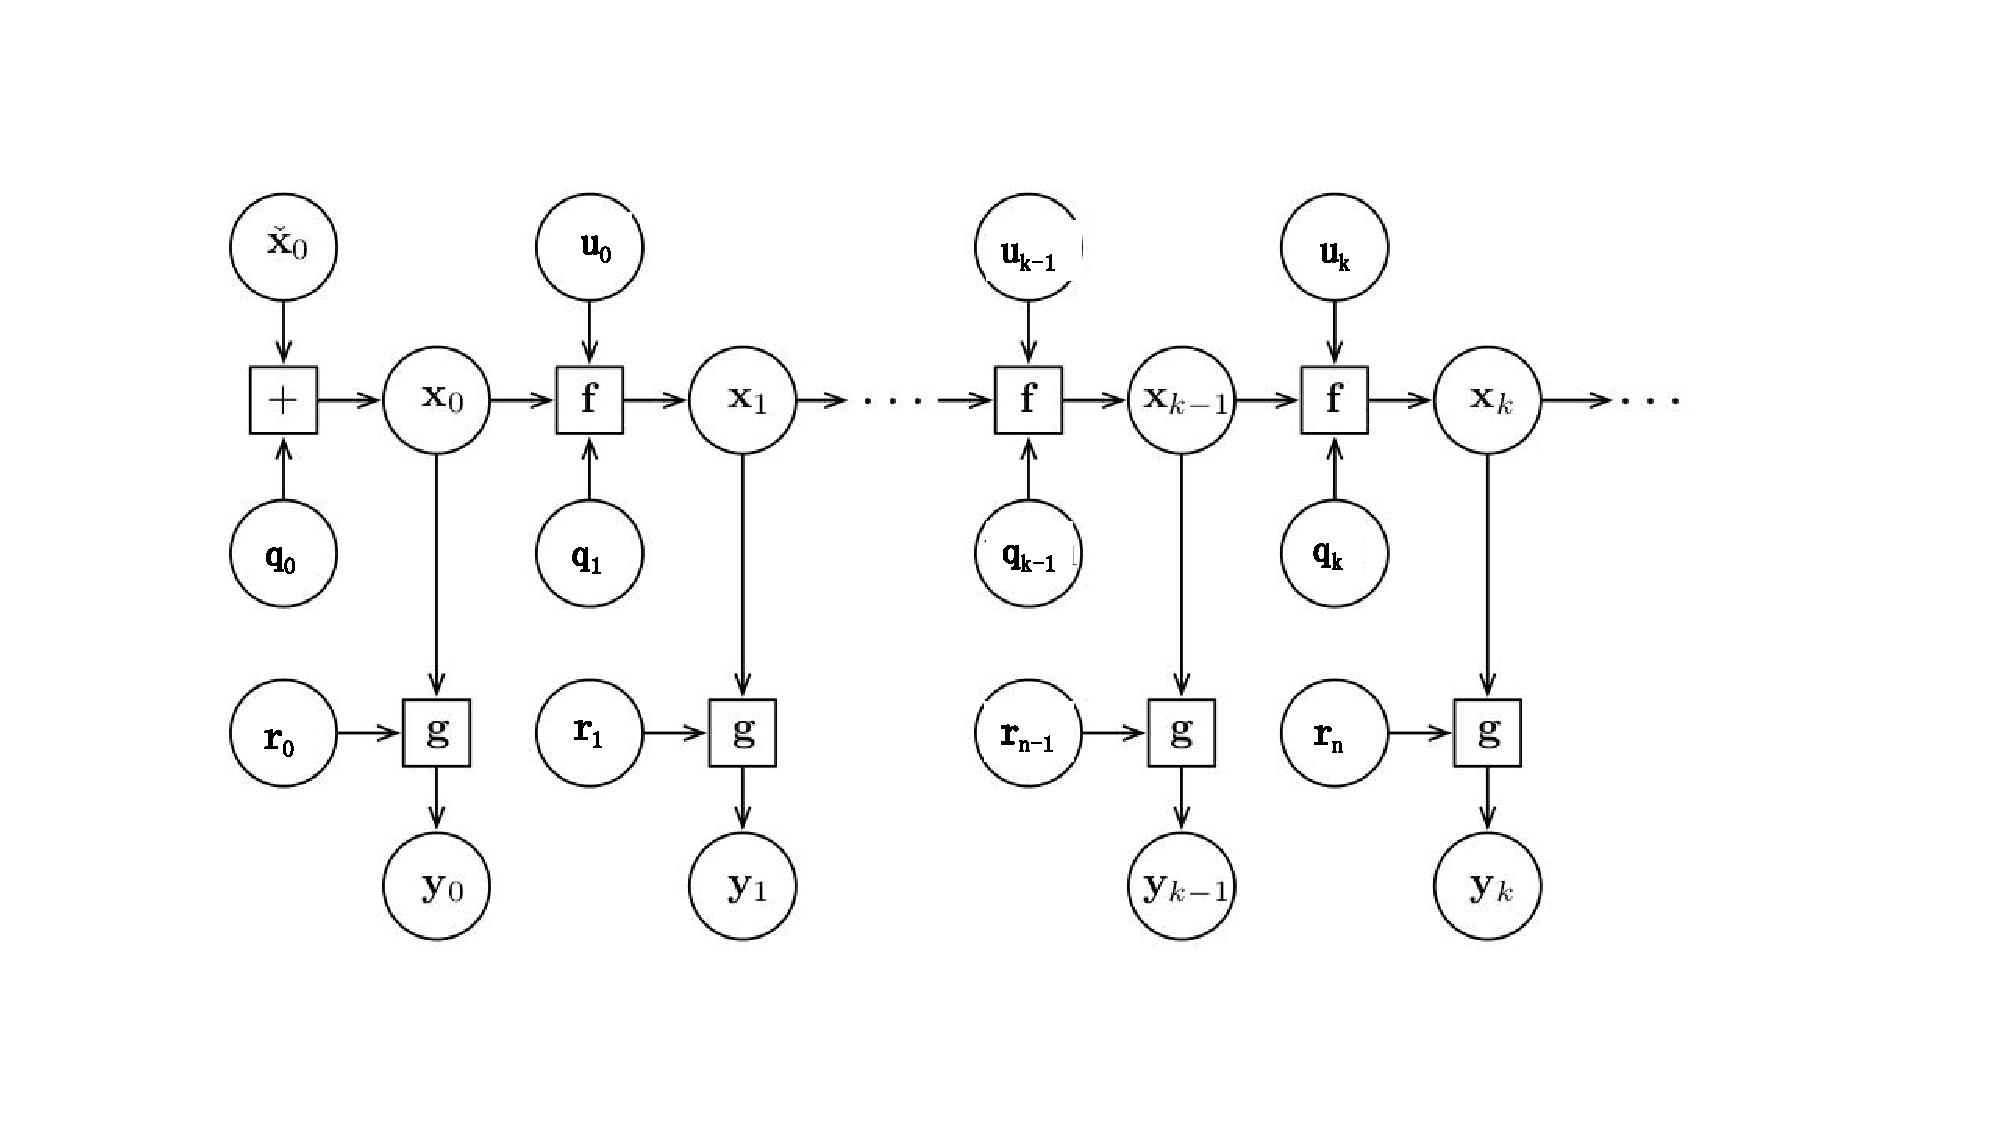
\includegraphics[width=0.45\linewidth]{state2.pdf}
\end{figure}
\end{frame}


\begin{frame}
\frametitle{Linear State Space Model}
\small
\begin{equation*}
\begin{cases}
\mathbf{x}_k=\mathbf{A}_{k}\mathbf{x}_{k-1}+\mathbf{B}_{k}\mathbf{u}_{k}+\mathbf{q}_{k}\\
\mathbf{y}_k=\mathbf{H}_k\mathbf{x}_k+\mathbf{r}_k
\end{cases}
\end{equation*}
\pause
\begin{equation*}
\begin{split}
\text{system state:}\quad&\mathbf{x}_k\in\mathbb{R}^N\\
\text{input state:}\quad &\mathbf{u}_k\in\mathbb{R}^N\\
\text{process noise:}\quad &\mathbf{q}_k\in\mathbb{R}^N\sim \mathcal{N}(\mathbf{0},\mathbf{Q}_k)\\
\text{measurement:}\quad& \mathbf{y}_k\in\mathbb{R}^M\\
\text{measurement noise:}\quad& \mathbf{r}_k\in\mathbb{R}^M\sim \mathcal{N}(\mathbf{0},\mathbf{R}_k)\\
\end{split}
\end{equation*}
\end{frame}


\begin{frame}
\frametitle{Linear State Space Model}
\small
\begin{equation*}
\begin{cases}
\mathbf{x}_k=\mathbf{A}_{k}\mathbf{x}_{k-1}+\mathbf{B}_{k}\mathbf{u}_{k}+\mathbf{q}_{k}\\
\mathbf{y}_k=\mathbf{H}_k\mathbf{x}_k+\mathbf{r}_k
\end{cases}
\end{equation*}
\pause
\begin{equation*}
\begin{split}
\text{transition matrix:}\quad& \mathbf{A}_k\in\mathbb{R}^{N\times N}\\
\text{control-input matrix:}\quad& \mathbf{B}_k\in\mathbb{R}^{N\times N}\\
\text{observation matrix:}\quad& \mathbf{H}_k\in\mathbb{R}^{M\times N}\\
\end{split}
\end{equation*}
\end{frame}



\subsection{Kalman Filter}


%\begin{frame}
%\frametitle{Filter Hypothesis}
%\small
%\flushleft
%\begin{enumerate}
%\item Kalman filter hypothesis:
%\begin{itemize}
%\item The dynamic system is linear.
%\item The noise is a Gaussian distribution.
%\item Posterior probability is a Gaussian distribution.
%\end{itemize}
%\item The expansion of Kalman filter:
%\begin{itemize}
%\item Non-linear: EKF, UKF.
%\item Non-linear, Non-Gaussian: Particle Filter.
%\end{itemize}
%\end{enumerate}
%\end{frame}


\begin{frame}
\frametitle{Kalman Filter}
\small
{\bf{Predict}}
\begin{equation*}
\begin{split}
\text{Predicted state estimate} \quad \hat{\mathbf{x}}_{k\mid k-1} &= \mathbf{A}_k\hat{\mathbf{x}}_{k-1\mid k-1} + \mathbf{B}_k \mathbf{u}_k +\mathbf{q}_{k}\\
\text{Predicted estimate covariance} \quad\mathbf{P}_{k\mid k-1} &=  \mathbf{A}_k \mathbf{P}_{k-1\mid k-1} \mathbf{A}_k^\mathrm{T} + \mathbf{Q}_k\\
\text{measurement residual}\quad \tilde{\mathbf{y}}_k &= \mathbf{z}_k - \mathbf{H}_k\hat{\mathbf{x}}_{k\mid k-1}\\
\end{split}
\end{equation*}
\pause
{\bf{Update}}
\begin{equation*}
\begin{split}
\text{residual covariance}\quad\mathbf{S}_k& = \mathbf{H}_k \mathbf{P}_{k\mid k-1} \mathbf{H}_k^\mathrm{T} + \mathbf{R}_k \\
\text{ ''Optimal'' Kalman gain }\quad \mathbf{K}_k &= \mathbf{P}_{k\mid k-1}\mathbf{H}_k^\mathrm{T} \mathbf{S}_k^{-1}\\
\text{Updated state estimate}\quad \hat{\mathbf{x}}_{k\mid k} &= \hat{\mathbf{x}}_{k\mid k-1} + \mathbf{K}_k\tilde{\mathbf{y}}_k\\
\text{Updated estimate covariance}\quad\mathbf{P}_{k|k} &= (\mathbf{I} - \mathbf{K}_k \mathbf{H}_k) \mathbf{P}_{k|k-1} \\
\end{split}
\end{equation*}
\end{frame}



%%%%begin from it tomorrow
\subsection{Extended Kalman Filter}


\begin{frame}
\frametitle{EKF-Nonlinear State Space Model} \small
\begin{equation*}
\begin{cases}
\mathbf{x}_k=\mathbf{f}(\mathbf{x}_{k-1},\mathbf{u}_{k},\mathbf{q}_{k})\\
\mathbf{y}_k=\mathbf{g}(\mathbf{x}_k,\mathbf{r}_k)
\end{cases}
\end{equation*}
\begin{equation*}
\begin{split}
\text{transition model:}\quad& \mathbf{f}\\
\text{observation model:}\quad& \mathbf{g}\\
\end{split}
\end{equation*}
\pause
\begin{equation*}
\begin{split}
\mathbf{f}(\mathbf{x}_{k-1},\mathbf{u}_{k},\mathbf{q}_{k})&\approx\check{\mathbf{x}}_k+\mathbf{A}_{k-1}(\mathbf{x}_{k-1}-\check{\mathbf{x}}_{k-1})+\mathbf{q}'_k\\
\mathbf{g}(\mathbf{x}_{k},\mathbf{u}_{k},\mathbf{r}_{k})&\approx\check{\mathbf{y}}_k+\mathbf{H}_{k}(\mathbf{x}_{k}-\check{\mathbf{x}}_{k})+\mathbf{r}'_k
\end{split}
\end{equation*}
\end{frame}


\begin{frame}
\small
\frametitle{EKF}{}
\small
{\bf{Predict}}
\begin{equation*}
\begin{split}
\text{Predicted state estimate} \quad \hat{\mathbf{x}}_{k\mid k-1} &= \mathbf{f}(\mathbf{x}_{k-1},\mathbf{u}_{k},\mathbf{q}_{k})\\
\text{Predicted estimate covariance} \quad\mathbf{P}_{k\mid k-1} &=  \mathbf{A}_k \mathbf{P}_{k-1\mid k-1} \mathbf{A}_k^\mathrm{T} + \mathbf{Q}'_k\\
\text{measurement residual}\quad \tilde{\mathbf{y}}_k &= \mathbf{z}_k - \mathbf{g}(\mathbf{x}_k,\mathbf{r}_k)\\
\end{split}
\end{equation*}
\pause
{\bf{Update}}
\begin{equation*}
\begin{split}
\text{residual covariance}\quad\mathbf{S}_k& = \mathbf{H}_k \mathbf{P}_{k\mid k-1} \mathbf{H}_k^\mathrm{T} + \mathbf{R}_k \\
\text{ ''Optimal'' Kalman gain }\quad \mathbf{K}_k &= \mathbf{P}_{k\mid k-1}\mathbf{H}_k^\mathrm{T} \mathbf{S}_k^{-1}\\
\text{Updated state estimate}\quad \hat{\mathbf{x}}_{k\mid k} &= \hat{\mathbf{x}}_{k\mid k-1} + \mathbf{K}_k\tilde{\mathbf{y}}_k\\
\text{Updated estimate covariance}\quad\mathbf{P}_{k|k} &= (\mathbf{I} - \mathbf{K}_k \mathbf{H}_k) \mathbf{P}_{k|k-1} \\
\end{split}
\end{equation*}
\end{frame}


\subsection{Particle Filter}

%\begin{frame}
%\small \frametitle{Particle Filter} {\bf{Other names of particle filters:}}
%\begin{itemize}
%\item Condensation Algorithms
%\item Sequential sampling-importance re-sampling(SIR)
%\item Bootstrap Filtering
%\item Interacting particle approximations
%\item Survival of the fittest
%\item ......
%\end{itemize}
%\end{frame}



\begin{frame}
\small \frametitle{Particle Filter}
\begin{itemize}
\item Sequential Monte Carlo Algorithm Based on Bayesian Criterion
\item Looking for a set of discrete sample points to approximate the
    probability density function
\end{itemize}
\end{frame}


\begin{frame}
\small \frametitle{Particle Filter-Monte Carlo}
\begin{itemize}
\item Estimate integral values (p is a gaussian distribution)
\begin{equation*}
v = \int_{-\infty}^{+\infty}{x^2p(x)dx}
\end{equation*}
\end{itemize}
\begin{itemize}
\item Monte Carlo:
\begin{enumerate}
\item Simulate M random variables
\begin{equation*}
x^{(m)}\sim N(0,\sigma^2)
\end{equation*}
\item Calculate the mean
\begin{equation*}
v = \frac{1}{M}\sum_{m=1}^{M}{(x^{(m)})}^2
\end{equation*}
\end{enumerate}
\end{itemize}
\end{frame}

\begin{frame}
\small \frametitle{Particle Filter-Importance sampling}
\begin{itemize}
\item Integral calculation
\begin{equation*}
E(f(x)) = \int_{-\infty}^{+\infty}{f(x)p(x)dx}= \int_{-\infty}^{+\infty}{f(x)\frac{p(x)}{\pi (x)}\pi (x)dx}
\end{equation*}
\end{itemize}
\begin{itemize}
\item Monte Carlo:
\begin{enumerate}
\item Simulate M random variables $\:(\pi (x))$
\begin{equation*}
x^{(m)}\sim \pi(x)
\end{equation*}
\item Calculate the expectation
\begin{equation*}
E(f(x))\thickapprox  \frac{1}{M}\sum_{m=1}^{M}{f(x^{(m)}) \underbrace{\frac{p(x^{(m)})}{\pi(x^{(m)})}}_{w^{(m)}}}
\end{equation*}
\end{enumerate}
\end{itemize}
\end{frame}

\begin{frame}
\small \frametitle{Particle Filter-Importance sampling}
\begin{itemize}
\item Integral calculation
\begin{equation*}
\begin{split}
&E(g_t(x_{0:t})) = \int{g_t(x_{0:t})p(x_{0:t}|y_{1:t})dx_{0:t}} \\
&E(g_t(x_{0:t})) = \int{g_t(x_{0:t})\frac {p(x_{0:t}|y_{1:t})}{q(x_{0:t}|y_{1:t})}q(x_{0:t}|y_{1:t})dx_{0:t}}
\end{split}
\end{equation*}
\item Monte Carlo:
\begin{enumerate}
\item Simulate M random variables $\:(q(x))$
\item Calculate the mean
\end{enumerate}
\end{itemize}
\begin{equation*}
E(g_t(x_{0:t}))= \frac{\frac{1}{M}\sum_{i=1}^{M} g_t(x_{0:t}^{(i)})w_t(x_{0:t}^{(i)})}{\frac{1}{M}\sum_{i=1}^{M} w_t(x_{0:t}^{(i)})}=\sum_{i=1}^{M}g_t(x_{0:t}^{(i)})\tilde{w}_t(x_{0:t}^{(i)})
\end{equation*}
\begin{equation*}
\hat{p}(x_{0:t}|y_{1:t})= \sum_{i=1}^{M} \int \tilde{w}_t^{(i)} \delta_{x_{0:t}^{(i)}}(dx_{0:t})
\end{equation*}
\end{frame}


\begin{frame}
\small \frametitle{Particle Filter-Sequential Importance Sampling}
\begin{equation*}
p(x_{0:t})=p(x_0)\prod_{j=1}^{t}p(x_j|x_{j-1}), \quad p(y_{1:t}|x_{0:t})=\prod_{j=1}^{t}p(y_j|x_{j})
\end{equation*}
\begin{equation*}
\begin{split}
&\text{1. \: Predicted state estimate}\quad x_k^{(m)} =p(x_k|x_{k-1}) \\
&\text{2a. \: Weight computation} \quad w_k^{*(m)} =w_{k-1}^{*(m)} p(y_k|x_k^{(m)}) \\
&\text{2b. \: Weight normalization} \quad w_k^{(m)} =\frac {w_{k}^{*(m)}}{\sum _{m=1}^{M}w_{k}^{*(m)}} \\
&\text{3. \: Estimation} \quad E(g(x_k|y_{1:k}))=\sum_{m=1}^{M}g(x_k^{(m)})w_k^{(m)} \\
\end{split}
\end{equation*}
\end{frame}

\begin{frame}
\small \frametitle{Particle Filter-Resampling}
\begin{figure}
\centering
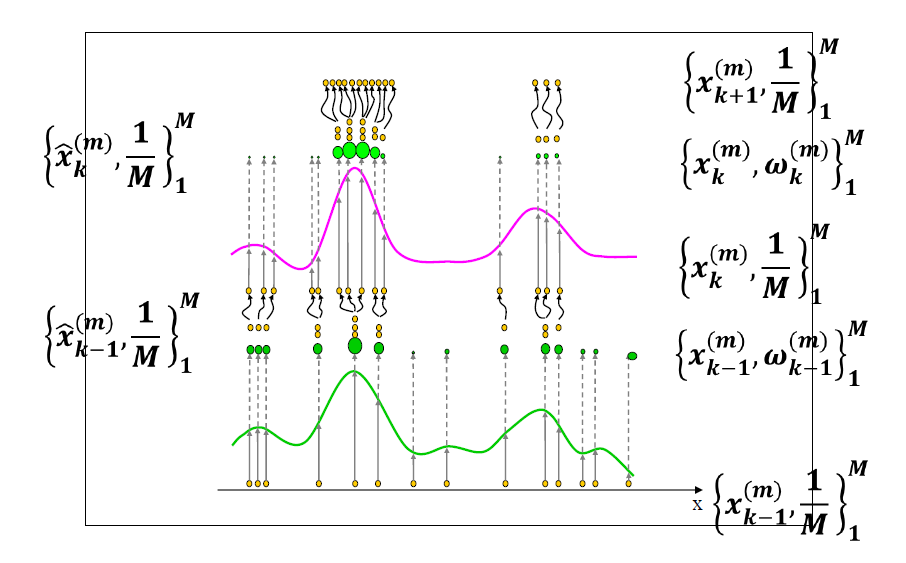
\includegraphics[width=1\linewidth]{resampling.png}
\end{figure}
\end{frame}

\begin{frame}
\small \frametitle{Particle Filter}{} \small {\bf{Advantages}}
\begin{itemize}
\item Global approximation.
\item Wide adaptability.
\end{itemize}\pause {\bf{Disadvantages}}
\begin{itemize}
\item Computational requirements much higher than of the Kalman filters.
\item Problems with nearly noise-free models, especially with accurate dynamic models.
\item The selection of particle numbers and important density function. 
\end{itemize}
\end{frame}


\section{Applications}
\frame{\tableofcontents[currentsection]}


\subsection{Tracking}

\begin{frame}
\frametitle{Tracking}\small
\begin{columns}
\column{0.5\textwidth}
red-observationbearing
green-velocty
blue(left)-EKF covariance
blue(right)-Particles
Comparison:
Accuracy
performance
\column{0.5\textwidth}
\begin{figure}
\centering
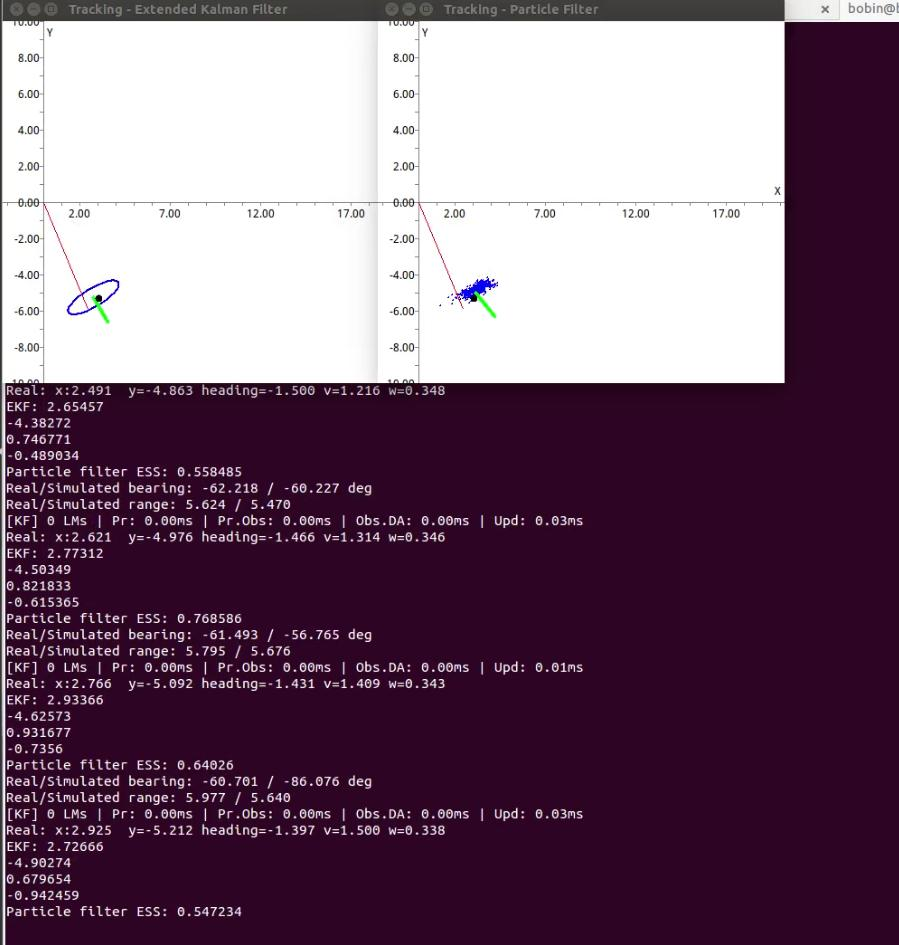
\includegraphics[width=1\linewidth]{tracking.jpg}
\end{figure}
\end{columns}
\end{frame}


\subsection{SLAM (Simultaneous Localization And Mapping)}

\begin{frame}{Hector SLAM}
\begin{figure}
\centering
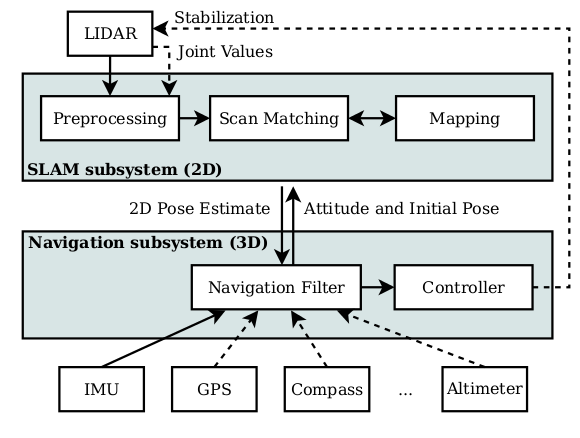
\includegraphics[width=0.5\linewidth]{hector-slam-system.png}
\end{figure}
\begin{itemize}\tiny
\item Kohlbrecher S, Von Stryk O, Meyer J, et al. A flexible and scalable slam system with full 3d motion estimation[C]//Safety, Security, and Rescue Robotics (SSRR), 2011 IEEE International Symposium on. IEEE, 2011: 155-160.
\end{itemize}
\end{frame}


\begin{frame}{Hector SLAM}
3D state
\begin{equation*}
\mathbf{x}=\begin{bmatrix}
\Omega^T & \mathbf{p}^T & \mathbf{v}^T
\end{bmatrix}
\end{equation*}
where
\begin{equation*}
\begin{split}
\Omega=\begin{bmatrix}
\phi,\theta,\varphi
\end{bmatrix} &\quad
\text{roll, pitch and yaw Euler angles}\\
\mathbf{p}=\begin{bmatrix}
\mathbf{p}_x,\mathbf{p}_y,\mathbf{p}_z
\end{bmatrix} &\quad
\text{posotion}\\
\mathbf{v}=\begin{bmatrix}
\mathbf{v}_x,\mathbf{v}_y,\mathbf{v}_z
\end{bmatrix} &\quad
\text{velocity}
\end{split}
\end{equation*}
\begin{itemize}\tiny
\item Kohlbrecher S, Von Stryk O, Meyer J, et al. A flexible and scalable slam system with full 3d motion estimation[C]//Safety, Security, and Rescue Robotics (SSRR), 2011 IEEE International Symposium on. IEEE, 2011: 155-160.
\end{itemize}
\end{frame}


\begin{frame}{Hector SLAM}
\begin{block}{Dynamic system}\small
\begin{equation*}
\begin{split}
\dot{\Omega}&=\mathbf{E}_\omega\cdot\omega\\
\dot{\mathbf{p}}&=\mathbf{v}\\
\dot{\mathbf{v}}&=\mathbf{R}_\omega\cdot\mathbf{a}+\mathbf{g}
\end{split}
\end{equation*}
where\scriptsize
\begin{equation*}
\begin{split}
\mathbf{R}_\omega \quad & \text{Rotation matrix from Sensor to world}\\
\mathbf{E}_\omega \quad & \text{maps angular rates to the derivatives of the Euler angles}\\
\mathbf{g} \quad & \text{constant gravity vector}
\end{split}
\end{equation*}
\begin{itemize}\tiny
\item Kohlbrecher S, Von Stryk O, Meyer J, et al. A flexible and scalable slam system with full 3d motion estimation[C]//Safety, Security, and Rescue Robotics (SSRR), 2011 IEEE International Symposium on. IEEE, 2011: 155-160.
\end{itemize}
\end{block}
\end{frame}

\begin{frame}
\frametitle{Hector SLAM}
\begin{figure}
\centering
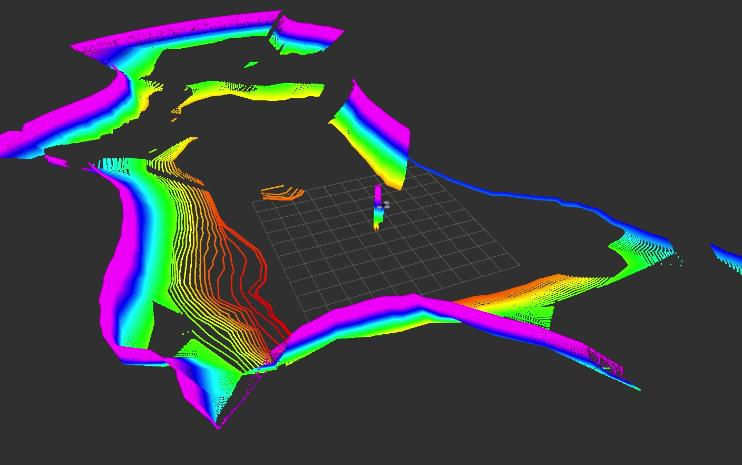
\includegraphics[width=0.6\linewidth]{hector-slam.jpg}
\end{figure}
\begin{itemize}\tiny
\item Kohlbrecher S, Von Stryk O, Meyer J, et al. A flexible and scalable slam system with full 3d motion estimation[C]//Safety, Security, and Rescue Robotics (SSRR), 2011 IEEE International Symposium on. IEEE, 2011: 155-160.
\end{itemize}
\end{frame}
\subsection{Inertial Navigation}


%\begin{frame}{Multi-Sensor Fusion}
%\begin{figure}
%\centering
%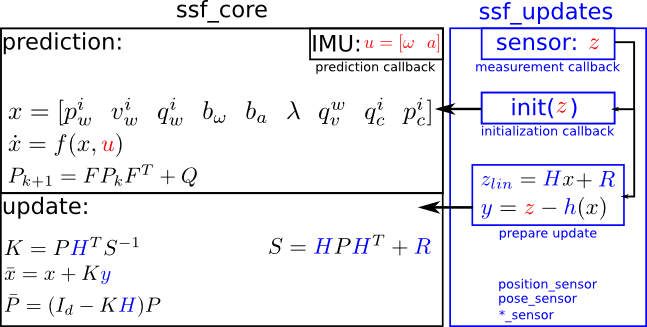
\includegraphics[width=0.5\linewidth]{msf-structure.png}
%\\\quad\\
%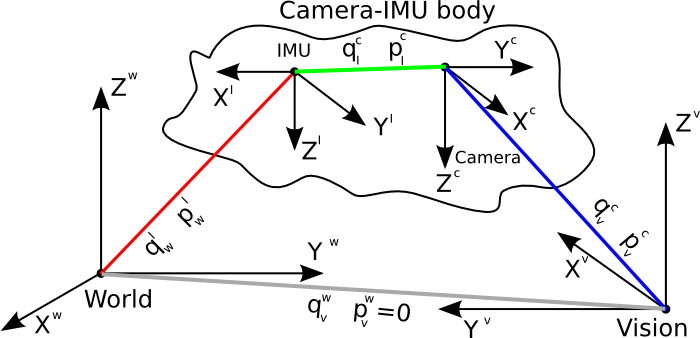
\includegraphics[width=0.5\linewidth]{framesetup.png}
%\end{figure}
%\begin{itemize}\tiny
%\item Stephan Weiss, Markus W. Achtelik, Margarita Chli and Roland Siegwart. Versatile Distributed Pose Estimation and Sensor Self-Calibration for Autonomous MAVs. in IEEE International Conference on Robotics and Automation (ICRA), 2012. pdf
%\item Stephan Weiss, Davide Scaramuzza and Roland Siegwart, Monocular-SLAM–based navigation for autonomous micro helicopters in GPS-denied environments, Journal of Field Robotics (JFR), Vol. 28, No. 6, 2011, 854-874. pdf
%\end{itemize}
%\end{frame}

%\begin{frame}{Multi-Sensor Fusion}
%\begin{figure}
%\centering
%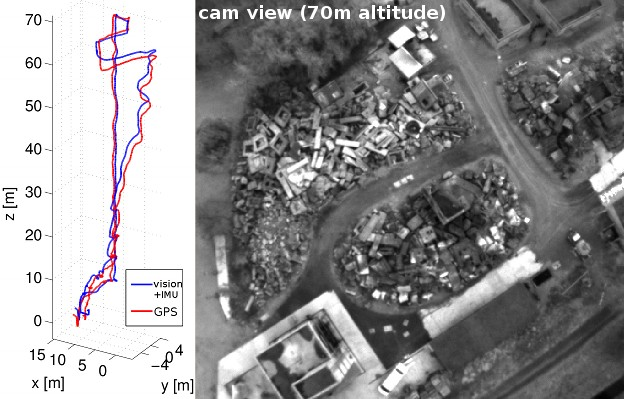
\includegraphics[width=0.5\linewidth]{ethzasl_ptam_icarus.jpg}
%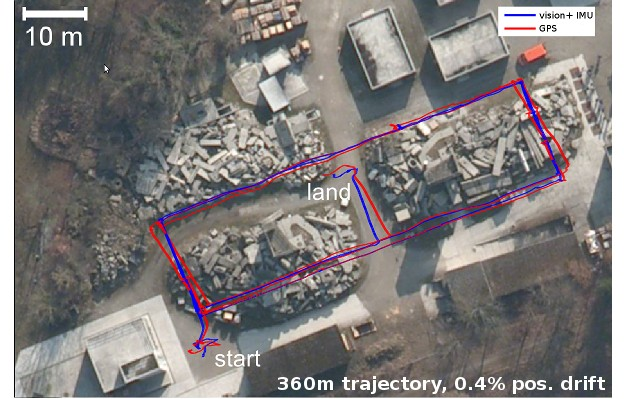
\includegraphics[width=0.5\linewidth]{ethzasl_ptam_traj.jpg}
%\end{figure}
%\begin{itemize}\tiny
%\item Stephan Weiss, Markus W. Achtelik, Margarita Chli and Roland Siegwart. Versatile Distributed Pose Estimation and Sensor Self-Calibration for Autonomous MAVs. in IEEE International Conference on Robotics and Automation (ICRA), 2012. pdf
%\item Simon Lynen, Markus Achtelik, Stephan Weiss, Margarita Chli and Roland Siegwart, A Robust and Modular Multi-Sensor Fusion Approach Applied to MAV Navigation. in Proc. of the IEEE/RSJ Conference on Intelligent Robots and Systems (IROS), 2013.
%\end{itemize}
%\end{frame}


\begin{frame}
\Huge
\begin{center}
Thank you
\end{center}
\end{frame}


\end{document}
